\section{Evaluation}
\label{sec:evaluation}
\label{Simulation Result}
\indent 
	We use simple version of signal modelling only considering path loss with some noise signal. 
\par 
	The following graphs are 4 simulation results that randomly allocate 4 robot objects and one signal power vs. distance simulation figure :\\
 
\begin{figure}[h]
\begin{minipage}[h]{0.4\linewidth}
	\centering
	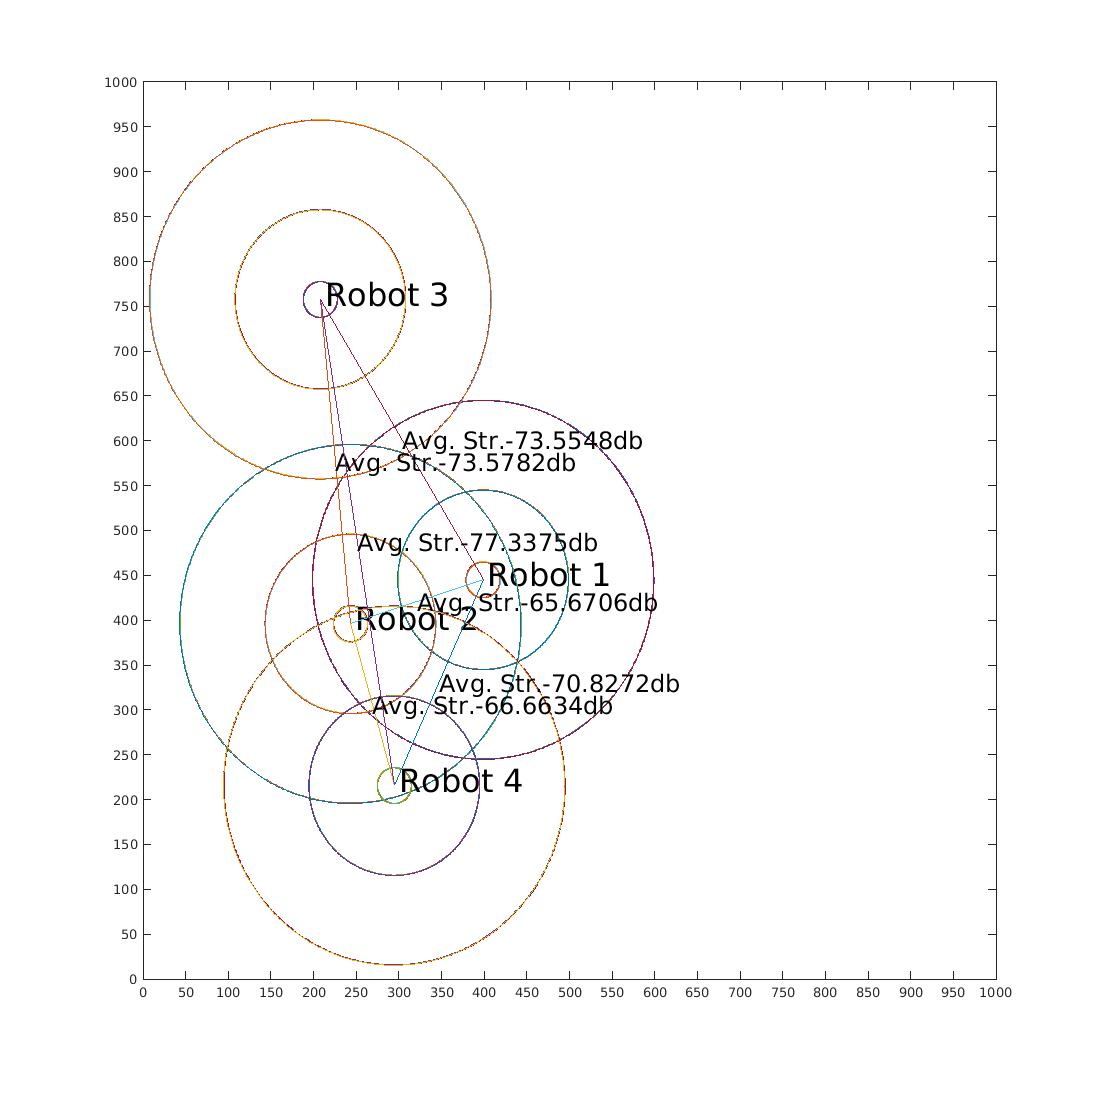
\includegraphics[width=\textwidth]{simulation1}
	\end{minipage}
	
	\begin{minipage}[h]{0.4\linewidth}
	\centering
	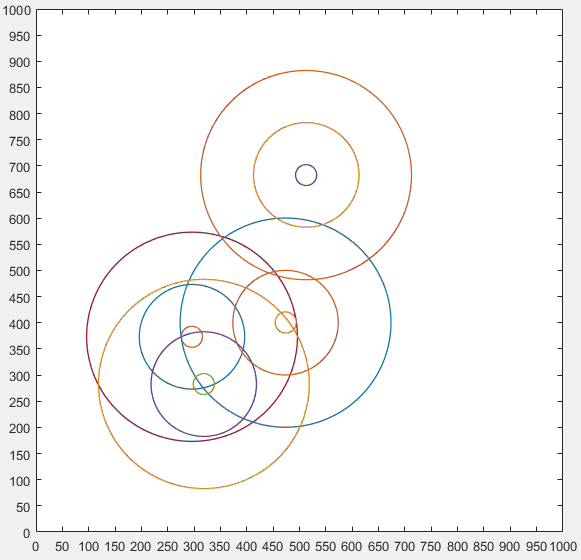
\includegraphics[width=\textwidth]{simulation2}
	\end{minipage}

	\begin{minipage}[h]{0.4\linewidth}
	\centering
	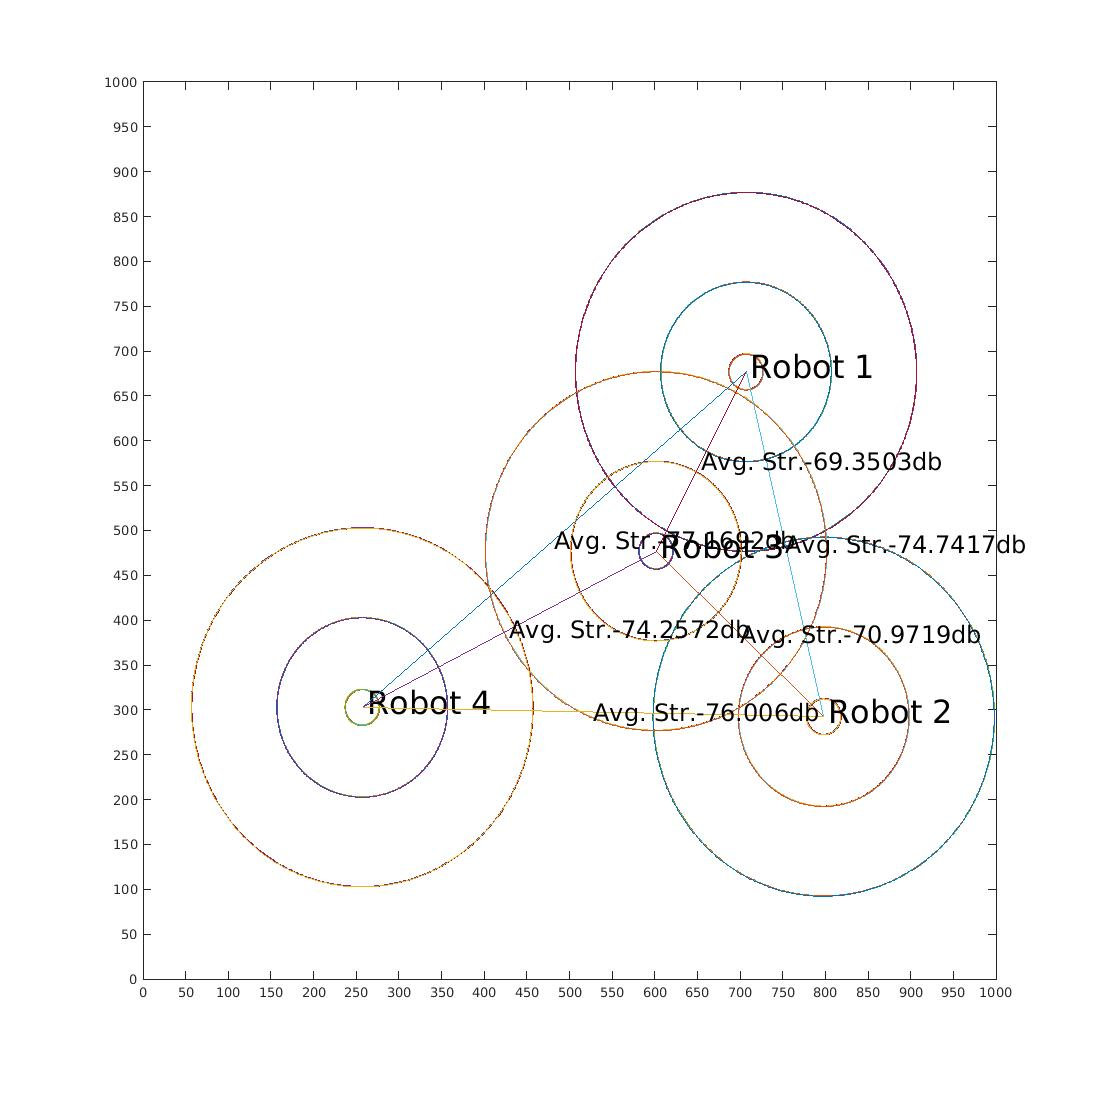
\includegraphics[width=\textwidth]{simulation3}
	\end{minipage}
	
	\begin{minipage}[h]{0.4\linewidth}
	\centering
	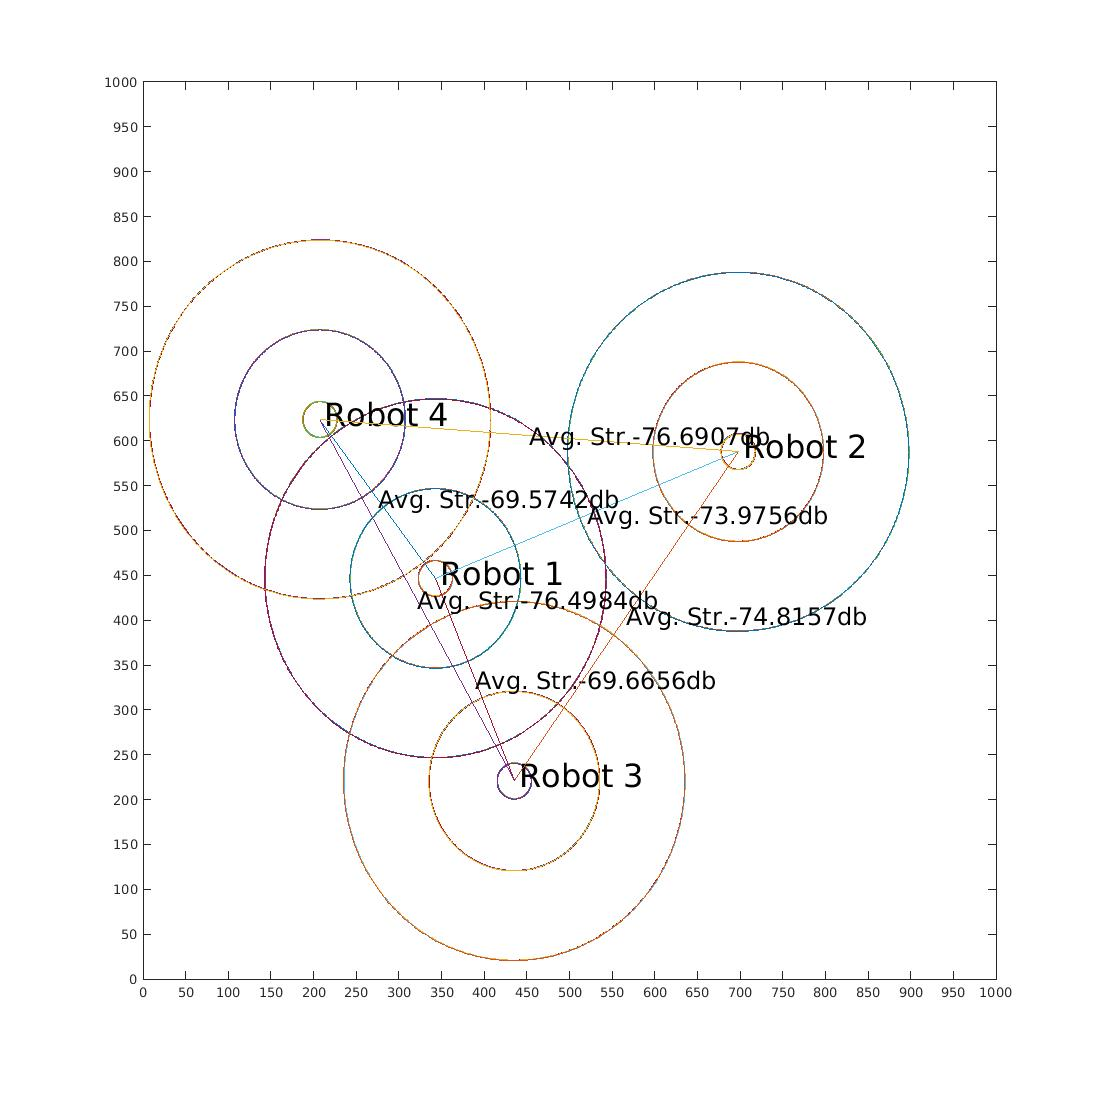
\includegraphics[width=\textwidth]{simulation4}
	\end{minipage}

\caption{Four sample simulations}

\begin{minipage}[h]{\linewidth}
	\centering
	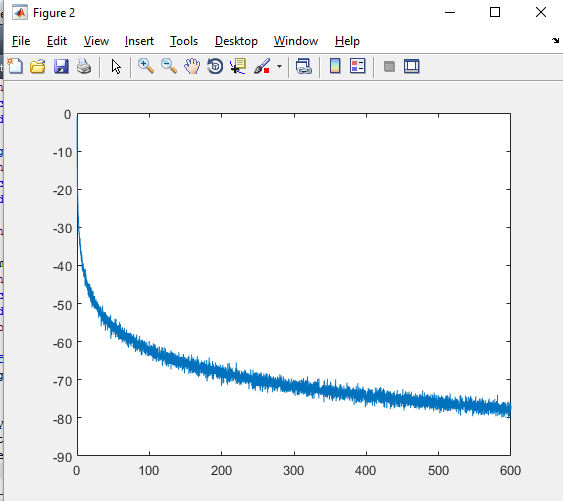
\includegraphics[width=\textwidth]{simulation5}
	\end{minipage}
	\caption{Power vs. Distance}
	
\label{fig:image2}
\end{figure}

